\documentclass{beamer}

% Packages 
\usepackage[utf8]{inputenc} % Input encoding 
\usepackage[T1]{fontenc} % Font encoding
\usepackage{amsmath,amssymb}  % For math
\usepackage{mathtools,nccmath,bbm} % Math extensions

\usepackage{comment} % Comment blocks

\usepackage{xcolor} % Color extensions
\usepackage{graphicx} % For figures
\usepackage[many]{tcolorbox} % For boxes

\usepackage{booktabs} % For tables

% Get rid of the navigation symbols 
\beamertemplatenavigationsymbolsempty

% Space between columns
\setlength{\columnsep}{0cm}

% Space below equations
\setlength{\belowdisplayskip}{0pt}

% Colorblind friendly palette

%% See https://mirrors.ibiblio.org/CTAN/macros/latex/contrib/beamer-contrib/themes/beamercolorthemeowl/beamercolorthemeowl.pdf

%% Primary -- use two or three
\definecolor{fmag}{RGB}{255,92,168} % Fancy magenta
\definecolor{fgre}{RGB}{90,168,0} % Fancy green
\definecolor{fblu}{RGB}{0,152,233} % Fancy blue
\definecolor{fyel}{RGB}{242,147,24} % Fancy yellow

%% Secondary -- just in case
\colorlet{fvio}{fmag!50!fblu} % Fancy violet
\colorlet{fbro}{fmag!50!fgre} % Fancy brown
\colorlet{fora}{fmag!50!fyel} % Fancy orange
\colorlet{fcya}{fgre!50!fblu} % Fancy cyan

% Maths default colors
\everymath{\color{black}} % \(\)
\everydisplay{\color{black}} % \[\]

% Buttons colors
\setbeamercolor{button}{bg=fblu,fg=white}

% Title color
\setbeamercolor*{title}{fg=fblu}  

% Title font family and weight
\setbeamerfont{title}{
    series=\bfseries,
    parent=structure,
    family=\rmfamily
}

% Subtitle color
\setbeamercolor*{subtitle}{fg=fblu}  

% Subtitle font family and weight
\setbeamerfont{subtitle}{
    series=\bfseries,
    parent=structure,
    family=\rmfamily
} 

% Headers color
\setbeamercolor{frametitle}{fg=fblu}

% Headers font family and weight
\setbeamerfont{frametitle}{
    size=\Large,
    series=\bfseries,
    parent=structure,
    family=\rmfamily
}

% Subheaders color
\setbeamercolor{framesubtitle}{fg=fblu}

% Subheaders font family and weight
\setbeamerfont{framesubtitle}{
    size=\footnotesize,
    series=\bfseries,
    parent=structure,
    family=\rmfamily
}

% Items color
\setbeamercolor{itemize item}{fg=black}
\setbeamercolor{itemize subitem}{fg=fblu}

% Items shape
\setbeamertemplate{itemize item}[square]
\setbeamertemplate{itemize subitem}[circle]

% Title page
\title{The Opioid Crisis}
\subtitle{State Regulations and Labor Market Outcomes}
\date{\today}
\author{Guillermo Martínez Martínez}
\institute{CEMFI}

% Define item and transition environments 
% -- cheers to Paul Goldsmith-Pinkham

%% See: https://github.com/paulgp/beamer-tips/blob/master/slides.tex

% Item environment
\newenvironment{wideitemize}{
    \itemize\addtolength{\itemsep}{10pt}
    }{\enditemize}

% Enumerate environment
\setbeamertemplate{enumerate items}[square]
\setbeamercolor{item projected}{bg=fblu,fg=white}
\newenvironment{wideenumerate}{
    \enumerate\addtolength{\itemsep}{10pt}
    }{\endenumerate}

% Transition environment
\newenvironment{transitionframe}{
  \setbeamercolor{background canvas}{bg=fblu}
  \begin{frame}
  }{\end{frame}}

% Text boxes
\newtcolorbox{mybox}{
    sharpish corners, 
    colback = white, 
    colframe = fblu,
    boxrule = 0.25pt, % very thin, may not render properly (zoom in and out)
    toprule = 4.5pt,
    enhanced
}

\begin{document}

\begin{frame}

    \rmfamily % Font
    
    \titlepage 

\end{frame}



\section{Introduction}

\begin{frame}

    \frametitle{The Opioid Crisis} % Title
    \framesubtitle{}  % Subtitle
    \rmfamily % Font

    \begin{wideitemize}
        \item 110,000 Americans died in 2022 as a consequence of drug abuse
    \end{wideitemize}

    \begin{center}
        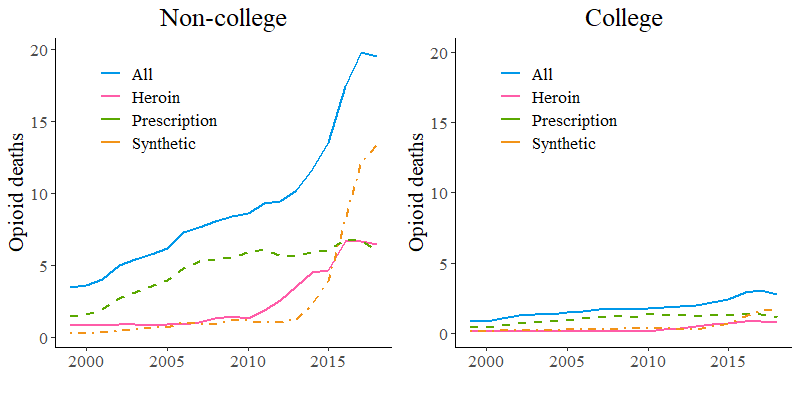
\includegraphics[scale=0.5]{ODD.png}
    \end{center}

    {\footnotesize \textit{Opioid deaths for both the non-college and college-educated as measured per 100,000 people in the respective education class (\textcolor{fgre}{Greenwood, Guner and Kopecky, 2022})}}
    
\end{frame}


\begin{frame}

    \label{Minimum Wage}
    \frametitle{State minimum wage trends} % Title
    \framesubtitle{}  % Subtitle
    \rmfamily % Font
    
    \begin{wideitemize} 
        \item States have been increasing their \textcolor{fblu}{minimum wage rates}, with varying intensity
    \end{wideitemize}

    \begin{center}
        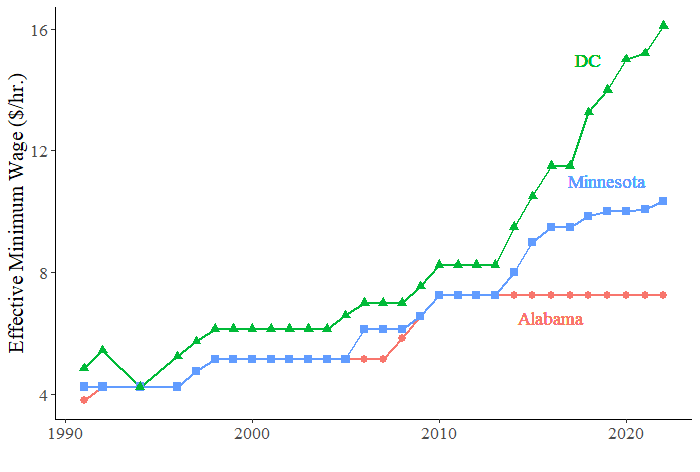
\includegraphics[scale=0.5]{min_wage_plot_simp.png}
    \end{center}
    
    \hyperlink{min_wage_plot_allstates}{\beamerbutton{All states}}
    
\end{frame}


\begin{frame}

    \frametitle{Main idea} % Title
    \framesubtitle{}  % Subtitle
    \rmfamily % Font
    
    \begin{wideitemize}
        \item Opioid misuse can lead the victims to negative labor market outcomes
        \item Minimum wage rates affect these outcomes 
        \vspace{9pt}
        \begin{wideitemize}
            \item[\textcolor{fblu}{\textbullet}] Negatively, through their impact on \textcolor{fblu}{labor demand for low-skill jobs} 
            \item[\textcolor{fblu}{\textbullet}] Positively, if they address the reasons that cause \textcolor{fblu}{addiction} in the first place \(\to\) \textcolor{fblu}{Deaths of despair}
        \end{wideitemize}
        \item The dominance of each effect depends on how \textcolor{fblu}{binding} minimum wage rates are across labor markets
    \end{wideitemize}

\end{frame}


\begin{frame}

    \frametitle{In this paper I ask} % Title
    \framesubtitle{}  % Subtitle
    \rmfamily % Font
    
    \begin{wideitemize}
        \item Do the effects of \textcolor{fblu}{Opioid Use Disorders} (\textcolor{fblu}{OUDs}) on labor market outcomes interact with minimum wage policies?
        \item If so, how have these policies shaped the ongoing Crisis?
        \item Is the interaction homogeneous across States, or can we expect differences across labor markets?
    \end{wideitemize}

    \vspace{9pt}
    I will use \textcolor{fblu}{changes in state prescription drug regulations} as a source of variation
    \vspace{9pt} 
    
    \begin{wideitemize}
        \item These changes can be seen as \textcolor{fblu}{exogeneous} from the \textcolor{fblu}{county level}
    \end{wideitemize}
    
\end{frame}


\begin{frame}

    \frametitle{Policy interactions} % Title
    \framesubtitle{}  % Subtitle
    \rmfamily % Font
    
    \begin{wideitemize}
        \item More stringent regulations on opioid access can make the victims to 
        \begin{wideitemize}
            \item[\textcolor{fblu}{\textbullet}] \textcolor{fblu}{Quit}, which might imply some disutility, or
            \item[\textcolor{fblu}{\textbullet}] \textcolor{fblu}{Switch to the black market}
        \end{wideitemize}
        \item This decision affects the MPL of the worker
        \item In this scenario, minimum wage increases can
        \vspace{9pt}
        \begin{wideitemize}
            \item[\textcolor{fblu}{\textbullet}] Improve labor outcomes if better living conditions tackle the causes of addiction and relapsing (\(\textcolor{fblu}{w_{min}}\) \textcolor{fblu}{not binding} after the change)
            \item[\textcolor{fblu}{\textbullet}] Foster addiction, if quitting doesn't improve employment prospects because \textcolor{fblu}{minimum wage becomes binding} 
        \end{wideitemize}
    \end{wideitemize}
    
\end{frame}

\begin{frame}

    \frametitle{Contribution} % Title
    \framesubtitle{}  % Subtitle
    \rmfamily % Font

    \begin{wideitemize}
        \item \textcolor{fgre}{Cengiz et al. (2019)} \(\to\) minimum wage changes reduced employment in low-wage jobs of tradeable sectors
        \item \textcolor{fgre}{Aliprantis, Fee, and Schweitzer (2023)} \(\to\) large and significant negative impact of prescription rates on labor force participation
        \item \textcolor{fgre}{Alpert, Powell, and Pacula (2018)} \(\to\) positive relation between OxyContin misuse and heroin deaths 
    \end{wideitemize}

    \vspace{9pt}
    \textbf{Contribution}: shedding light on how the policy responses to the \textcolor{fblu}{Opioid Crisis} have been affected by \textcolor{fblu}{minimum wage changes}
    \vspace{9pt}
    
    \begin{wideitemize}
        \item Interest in how \textcolor{fblu}{labor market regulations} interact with \textcolor{fblu}{Substance Abuse Disorders}
    \end{wideitemize}
    
\end{frame}



\section{Model}

\begin{transitionframe}

    \rmfamily % Font
    
    \begin{center}
    {\Huge \textbf{\textcolor{white}{Model}}}
    \end{center}
  
\end{transitionframe}

\begin{frame}

    \frametitle{Set Up} % Title
    \framesubtitle{}  % Subtitle
    \rmfamily % Font

    An addicted worker faces
    \vspace{9pt}
    \begin{wideitemize}
        \item A health/performance \textcolor{fblu}{cost of opioid consumption} \(O_{it}\)
        \item This cost depends on \textcolor{fblu}{legal opioids consumption} \(l_{it}\) and \textcolor{fblu}{black market opioids consumption} \(h_{it}\) (say, heroin)
        \item Which opioid is consumed depends on the \textcolor{fblu}{availability of legal opioids} \(z_{it}\) (\(= 1\) if prescription law is in place)
        \item I assume that illegal opioids are more harmful than legal opioids 
        \[h_{it} = l_{it} + \mathcal{C}\]
    \end{wideitemize}

\end{frame}

\begin{frame}

    \label{decision_making}
    \frametitle{Policy and decision making} % Title
    \framesubtitle{}  % Subtitle
    \rmfamily % Font

    \begin{wideitemize}
        \item The \textcolor{fblu}{total cost of opioid consumption} is
        \[
        O_{it} = z_{t}\left(1-q_{it}\right)h_{it} + (1-z_{t})l_{it}
        \]
        where \(q_{it} = 1\) \textcolor{fblu}{if the worker quits opioids}
        \item The worker quits if
        
        \[
        q_{it} = \mathbbm{1}\{\text{Exp. utility of quitting} \geq \text{Disutility of quitting}\}
        \]

    \end{wideitemize}
    \hyperlink{quitting}{\beamerbutton{Quitting}}    

\end{frame}


\begin{frame}

    \frametitle{Labor demand} % Title
    \framesubtitle{}  % Subtitle
    \rmfamily % Font

    \begin{wideitemize}
        \item The \textcolor{fblu}{representative firm} maximizes profits
        \[
        \pi_{it} = Y_{it} - w_{it}L_{it} \quad \text{s.t} \quad w_t \geq w^{min}_t
        \]
        \vspace{-15pt}
        \item The \textcolor{fblu}{MPL} is given by
        \[
        \dfrac{\partial Y_{it}}{\partial L_{it}} = f(\theta_{it}) - \kappa\cdot\mathbbm{1}\{O_{it}\geq o\}
        \]
        where \(\theta_{it}\) is the \textcolor{fblu}{worker's ability} and \(\kappa\) captures the \textcolor{fblu}{impact of addiction on productivity}
    \end{wideitemize}

\end{frame}


\begin{frame}

    \frametitle{Impact on labor market outcomes} % Title
    \framesubtitle{}  % Subtitle
    \rmfamily % Font

    \begin{wideitemize}
        \item Assume for the moment that \textcolor{fblu}{the worker cannot quit opioids} and that \(l_{it} < o < h_{it}\)
        \item Then if the \textcolor{fblu}{minimum wage is binding} (\(w_{t} = w^{min}_t\)) and \textcolor{fblu}{the law is passed} (\(z_t = 1\))
        \[
        f(\theta_{it}) - \kappa < w^{min}_t \,\Rightarrow\, \text{unemployment}
        \]
        \vspace{-15pt}
        \item But if the \textcolor{fblu}{minimum wage is not binding} (\(w_{t} >> w^{min}_t\)) 
        \[
        f(\theta_{it}) - \kappa = w_t 
        \]
        \vspace{-15pt}
        \item What if the worker can quit opioids?
    \end{wideitemize}
    \hyperlink{quitting}{\beamerbutton{Quitting}} 
\end{frame}





\section{Data}

\begin{transitionframe}

    \rmfamily % Font
    
    \begin{center}
    {\Huge \textbf{\textcolor{white}{Data}}}
    \end{center}
  
\end{transitionframe}

\begin{frame}

    \frametitle{Data I} % Title
    \framesubtitle{}  % Subtitle
    \rmfamily % Font

    \begin{wideitemize}
        \item \textcolor{fgre}{US Bureau of Labor Statistics (BLS)}  
        \vspace{9pt}
        \begin{wideitemize}
            \item[\textcolor{fgre}{\textbullet}] \textcolor{fgre}{LAUS Database} \(\to\) County-level labor market statistics (1990-2023)
            \item[\textcolor{fgre}{\textbullet}] \textcolor{fgre}{OEWS Database} \(\to\) National industry-specific occupations and wages statistics (1997-2023) % Occupational Employment and Wage Statistics
        \end{wideitemize}
        \item \textcolor{fgre}{Eckert et al. (2020)} \(\to\) County-level industry-specific employment (1975-2016) 
        \item \textcolor{fgre}{USDOL's Changes in Basic Minimum Wages} (1968-2023)
        \item \textcolor{fgre}{US Census Bureau's Population Estimates Program (PEP)} \(\to\) County-level population and demographics (1969-2020)
        \item \textcolor{fgre}{DEA's ARCOS} \(\to\) Opioid distribution data (2006-2014)
    \end{wideitemize}

\end{frame}


\begin{frame}

    \frametitle{Data II} % Title
    \framesubtitle{}  % Subtitle
    \rmfamily % Font

    \begin{wideitemize}
        \item \textcolor{fgre}{Horwitz et al. (2020)} \(\to\) Prescription Drug Monitoring Programs (1990-2019)
        \item \textcolor{fgre}{Centers for Disease Control (CDC)} 
        \vspace{9pt}
        \begin{wideitemize}
            \item[\textcolor{fgre}{\textbullet}] \textcolor{fgre}{National Vital Statistics System} \(\to\) Total drug poisoning mortality by county (2003-2021)
            \item[\textcolor{fgre}{\textbullet}] \textcolor{fgre}{Multiple Cause of Death} \(\to\) Overdose deaths at the state-year level, for different drugs (1999-2020)
        \end{wideitemize}
         
    \end{wideitemize}

    \vspace{9pt}
    Current working sample:
    \vspace{9pt}
    
    \begin{wideitemize}
        \item Unemployment, PDMPs, Minimum Wage rates and demographics for counties of 50 States + DC, 1998-2019
        \item County-level industry-weighted wage distribution and death mortality for counties of 50 States + DC, 2003-2016
    \end{wideitemize}

\end{frame}


\begin{frame}

    \frametitle{PDMPs} % Title
    \framesubtitle{}  % Subtitle
    \rmfamily % Font
    
    Prescription Drug Monitoring Programs (\textcolor{fblu}{PDMPs}): electronic database that tracks controlled substance prescriptions
    \vspace{9pt}

    \begin{wideenumerate}
        \item \textcolor{fblu}{Modern System PDMPs}: the electronic database becomes accessible to any authorized user (eg, physician, pharmacist, or member of law enforcement)
        \item \textcolor{fblu}{Must Query PDMPs}: the law mandates the prescriber to check the database before prescribing a listed opioid
    \end{wideenumerate}

    %\vspace{9pt}
    %2 always follows 1, but 1 does not always lead to 2
    

\end{frame}


\section{Estimation}

\begin{transitionframe}

    \rmfamily % Font
    
    \begin{center}
    {\Huge \textbf{\textcolor{white}{Estimation}}}
    \end{center}
  
\end{transitionframe}

\begin{frame}

    \frametitle{Kaitz-\(\textcolor{fblu}{\text{\(\rho\)}}\) index} % Title
    \framesubtitle{}  % Subtitle
    \rmfamily % Font
    
    \begin{wideitemize}
        \item Measure of minimum wage bindingness
    \end{wideitemize}
    
    \begin{equation*}
        \text{\textit{kaitz}}_{ct}(\rho) \equiv \log{w^{\text{\textit{min}}}_{ct}} - \log{w^{\rho}_{ct}}
    \end{equation*}
    with 
    \begin{equation*}
        w^{\rho}_{ct} = \sum_{i\in c} \dfrac{e_i}{E_c}\,w^{\rho}_{it} \quad\text{and}\quad w^{\rho}_{it} = \sum_{o\in i} \dfrac{e_o}{E_{it}}\,w^{\rho}_{oit}
    \end{equation*}
    and
    \vspace{9pt}
    \begin{wideitemize}
        \item[\textcolor{fblu}{\textbullet}] \(\textcolor{fblu}{w^{\text{\textit{min}}}_{ct}}\): minimum wage in county \(\textcolor{fblu}{c}\) at time \(\textcolor{fblu}{t}\), \(\textcolor{fblu}{w^{\rho}_{ct}}\): wage percentile \(\textcolor{fblu}{\rho}\)
        \item[\textcolor{fblu}{\textbullet}] \(\textcolor{fblu}{w^{\rho}_{cit}}\): wage percentile in occupation \(\textcolor{fblu}{o}\) in industry \(\textcolor{fblu}{i}\) at time \(\textcolor{fblu}{t}\) 
        \item[\textcolor{fblu}{\textbullet}] \(\textcolor{fblu}{e_o}\): share of employment of occupation \(\textcolor{fblu}{o}\) in industry \(\textcolor{fblu}{i}\), \(\textcolor{fblu}{e_i}\): share of county employment in industry \(\textcolor{fblu}{i}\)
    \end{wideitemize}
    
\end{frame}

\begin{frame}

    \frametitle{Kaitz-\(\textcolor{fblu}{\text{\(\rho\)}}\) index} % Title
    \framesubtitle{}  % Subtitle
    \rmfamily % Font

    \begin{center}
        \includegraphics[scale=0.5]{kaitz_percentiles.png}
    \end{center}

\end{frame}

\begin{frame}

    \frametitle{Empirical model} % Title
    \framesubtitle{}  % Subtitle
    \rmfamily % Font
    
    \begin{wideitemize}
        \item Individual-level event study: \textcolor{fgre}{Arkhangelsky, Yanagimoto and Zohar (2024)}
    \end{wideitemize}
    
    \begin{equation*}
        y_{ct} = \alpha_c + \lambda_t + \sum_{k\geq h}\tau_{ck} + \beta X_{ct} + \nu_{ct}
    \end{equation*}
    with 
    \vspace{9pt}
    \begin{wideitemize}
        \item[\textcolor{fblu}{\textbullet}] \(\textcolor{fblu}{c}\): county, \(\textcolor{fblu}{t}\): time (year-month), \(\textcolor{fblu}{k = t - z_c}\): time difference from PDMP implementation year in county \(\textcolor{fblu}{c}\), \(\textcolor{fblu}{z_c}\)
        \item[\textcolor{fblu}{\textbullet}] \(\textcolor{fblu}{y_{ct}}\): labor market outcome; \(\textcolor{fblu}{X_{ct}}\): demographic covariates, sector shares and drug mortality; \(\textcolor{fblu}{\nu_{ct}}\): idiosyncratic shock 
    \end{wideitemize}
    \vspace{9pt}
    State-level changes must be exogenous at the county level for \textcolor{fblu}{identification} and no anticipation up to \(\textcolor{fblu}{h}\) periods
    
\end{frame}

\begin{frame}

    \label{lab_force_rate_result}
    \frametitle{Results} % Title
    \framesubtitle{}  % Subtitle
    \rmfamily % Font
    
    \begin{center} % 
        %\includegraphics[scale=0.4]{mop10_lab_force_rate.png}
        \includegraphics[scale=0.4]{pmq10_lab_for_rate.png}
    \end{center}

    \hyperlink{perc_comparison_3}{\beamerbutton{Percentiles comparison}}
    \hyperlink{ta_3}{\beamerbutton{Time average}}
    \hyperlink{presc_3}{\beamerbutton{Prescriptions}}

\end{frame}

\begin{frame}

    \label{unemp_rate_result}
    \frametitle{Results} % Title
    \framesubtitle{}  % Subtitle
    \rmfamily % Font
    
    \begin{center} %pmq10_unemp_rate.png
        %\includegraphics[scale=0.4]{mop10_unemp_rate.png}
        \includegraphics[scale=0.4]{pmq10_unemp_rate.png}
    \end{center}

    \hyperlink{perc_comparison_1}{\beamerbutton{Percentiles comparison}}
    \hyperlink{ta_1}{\beamerbutton{Time average}}
    \hyperlink{presc_1}{\beamerbutton{Prescriptions}}

\end{frame}


\begin{frame}

    \label{emp_rate_result}
    \frametitle{Results} % Title
    \framesubtitle{}  % Subtitle
    \rmfamily % Font
    
    \begin{center} % pmq10_emp_rate.png
        %\includegraphics[scale=0.4]{mop10_emp_rate.png}
        \includegraphics[scale=0.4]{pmq10_emp_rate.png}
    \end{center}

    \hyperlink{perc_comparison_2}{\beamerbutton{Percentiles comparison}}
    \hyperlink{ta_2}{\beamerbutton{Time average}}
    \hyperlink{presc_2}{\beamerbutton{Prescriptions}}

\end{frame}

\begin{frame}

    \label{heroin_result}
    \frametitle{Results} % Title
    \framesubtitle{}  % Subtitle
    \rmfamily % Font
    
    \begin{center} % pmq10_emp_rate.png
        %\includegraphics[scale=0.4]{mop10_emp_rate.png}
        \includegraphics[scale=0.4]{pmq10_heroin.png}
    \end{center}

    \hyperlink{table_heroin}{\beamerbutton{Coefficients}}

\end{frame}


\begin{comment}

\begin{frame}

    \frametitle{What is to be done?} % Title
    \framesubtitle{}  % Subtitle
    \rmfamily % Font
    
    \begin{wideitemize}
        \item Minimum wage measures of bindingness
        \vspace{9pt}
        \begin{wideitemize}
            \item Idea: we can estimate the effect of minimum wage on employment for wage bins
            \item Then assign, if significant, the coefficient to each county
            \item Sector compositions of the counties can also be relevant
        \end{wideitemize}
        \item I'm \textcolor{fblu}{open to suggestions}
        \item Participation rates might capture some of the effect
        \item Distribution of individual effects
    \end{wideitemize}
    
\end{frame}

\end{comment}




\begin{transitionframe}

    \rmfamily % Font
    
    \begin{center}
    {\Huge \textbf{\textcolor{white}{Thank you!}}}
    \end{center}
  
\end{transitionframe}


\section{Appendix}

\begin{frame}

    \label{min_wage_plot}
    
    \frametitle{State minimum wage trends} % Title
    \framesubtitle{}  % Subtitle
    \rmfamily % Font
    
    \begin{wideitemize}
        \item States have been increasing their \textcolor{fblu}{minimum wage rates}, with varying intensity
    \end{wideitemize}

    \begin{center}
        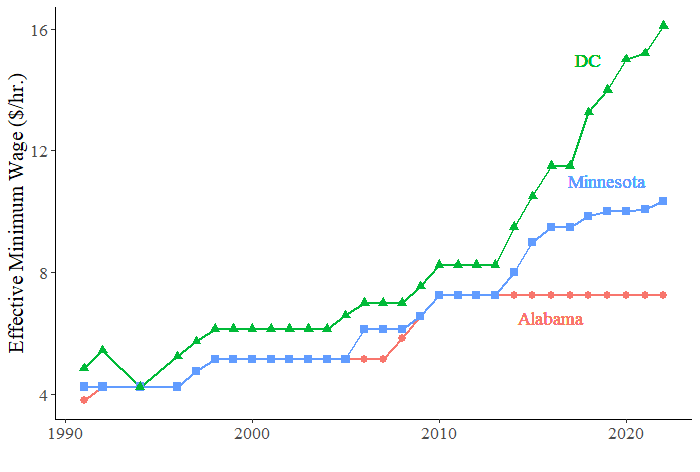
\includegraphics[scale=0.5]{min_wage_plot_simp.png}
    \end{center}
    
    \hyperlink{main_idea}{\beamerbutton{Back}}
    
\end{frame}

\begin{frame}

    \label{min_wage_plot_allstates}
    
    \frametitle{State minimum wage trends} % Title
    \framesubtitle{}  % Subtitle
    \rmfamily % Font
    
    \begin{wideitemize}
        \item States have been increasing their \textcolor{fblu}{minimum wage rates}, with varying intensity
    \end{wideitemize}

    \begin{center}
        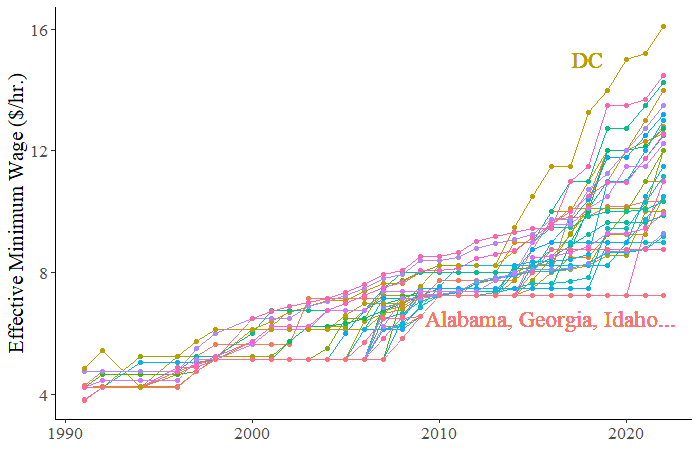
\includegraphics[scale=0.5]{min_wage_plot.png}
    \end{center}
    
    \hyperlink{main_idea}{\beamerbutton{Back}}
    
\end{frame}

\begin{comment}
\begin{frame}

    \label{quitting}
    \frametitle{Quitting decision I} % Title
    \framesubtitle{}  % Subtitle
    \rmfamily % Font

    \begin{wideitemize}
        \item Workers will quit opioids \textcolor{fblu}{if the expected utility of quitting is greater than the disutility of quitting} (\(\mathcal{C}_{quit}\))
        \item If the \textcolor{fblu}{minimum wage is not binding} and \textcolor{fblu}{the law is passed}
        \[
        q_{w_{it} > w^{min}_t} = \mathbbm{1}\{u\left(f(\theta_{it})L_{it}\right) - \mathcal{C}_{quit} \geq u\left(\left(f(\theta_{it}) - \kappa\right)L_{it}\right)\}
        \]
        \vspace{-15pt}
        \item If the \textcolor{fblu}{minimum wage is binding} and \textcolor{fblu}{the law is passed}
        \[
        q_{\,w_{it} = w^{min}_t} = \mathbbm{1}\{u\left(w^{min}_tL_{it}\right) - \mathcal{C}_{quit} \geq 0\}
        \]
    \end{wideitemize}
    
    \hyperlink{decision_making}{\beamerbutton{Back}}    

\end{frame}


\begin{frame}

    \frametitle{Quitting decision II} % Title
    \framesubtitle{}  % Subtitle
    \rmfamily % Font

    \begin{wideitemize}
        \item As long as
        \[
        u\left(f(\theta_{it})L_{it}\right) - u\left(\left(f(\theta_{it}) - \kappa\right)L_{it}\right) \geq \mathcal{C}_{quit} \geq u\left(w^{min}_tL_{it}\right)
        \]
        we should observe \textcolor{fblu}{more quitting where the minimum wage is less binding}
        \item This relation depends on \textcolor{fblu}{how much opioids affect productivity} and \textcolor{fblu}{how costly quitting is}
    \end{wideitemize}
    
    \hyperlink{decision_making}{\beamerbutton{Back}}    

\end{frame}
\end{comment}

\begin{frame}

    \label{perc_comparison_3}
    
    \frametitle{Percentiles comparison} % Title
    \framesubtitle{}  % Subtitle
    \rmfamily % Font

    \begin{center}
        \includegraphics[scale=0.4]{pmq10_lab_for_rate_comp6.png}
    \end{center}
    
    \hyperlink{lab_force_rate_result}{\beamerbutton{Back}}
    
\end{frame}

\begin{frame}

    \label{perc_comparison_31}
    
    \frametitle{Percentiles comparison} % Title
    \framesubtitle{}  % Subtitle
    \rmfamily % Font

    \begin{center}
        \includegraphics[scale=0.4]{pmq10_lab_for_rate_comp24.png}
    \end{center}
    
    \hyperlink{lab_force_rate_result}{\beamerbutton{Back}}
    
\end{frame}

\begin{frame}

    \label{perc_comparison_1}
    
    \frametitle{Percentiles comparison} % Title
    \framesubtitle{}  % Subtitle
    \rmfamily % Font

    \begin{center}
        \includegraphics[scale=0.4]{pmq10_unemp_rate_comp6.png}
    \end{center}
    
    \hyperlink{unemp_rate_result}{\beamerbutton{Back}}
    
\end{frame}

\begin{frame}

    \label{perc_comparison_12}
    
    \frametitle{Percentiles comparison} % Title
    \framesubtitle{}  % Subtitle
    \rmfamily % Font

    \begin{center}
        \includegraphics[scale=0.4]{pmq10_unemp_rate_comp24.png}
    \end{center}
    
    \hyperlink{unemp_rate_result}{\beamerbutton{Back}}
    
\end{frame}

\begin{frame}

    \label{perc_comparison_2}
    
    \frametitle{Percentiles comparison} % Title
    \framesubtitle{}  % Subtitle
    \rmfamily % Font

    \begin{center}
        \includegraphics[scale=0.4]{pmq10_emp_rate_comp6.png}
    \end{center}
    
    \hyperlink{emp_rate_result}{\beamerbutton{Back}}
    
\end{frame}

\begin{frame}

    \label{perc_comparison_21}
    
    \frametitle{Percentiles comparison} % Title
    \framesubtitle{}  % Subtitle
    \rmfamily % Font

    \begin{center}
        \includegraphics[scale=0.4]{pmq10_emp_rate_comp24.png}
    \end{center}
    
    \hyperlink{emp_rate_result}{\beamerbutton{Back}}
    
\end{frame}

\begin{frame}

    \label{ta_3}
    
    \frametitle{Time Averages} % Title
    \framesubtitle{}  % Subtitle
    \rmfamily % Font

    \begin{center}
        \includegraphics[scale=0.4]{pmq10_lab_for_rate_ta.png}
    \end{center}
    
    \hyperlink{lab_force_rate_result}{\beamerbutton{Back}}
    
\end{frame}

\begin{frame}

    \label{ta_1}
    
    \frametitle{Time Averages} % Title
    \framesubtitle{}  % Subtitle
    \rmfamily % Font

    \begin{center}
        \includegraphics[scale=0.4]{pmq10_unemp_rate_ta.png}
    \end{center}
    
    \hyperlink{unemp_rate_result}{\beamerbutton{Back}}
    
\end{frame}

\begin{frame}

    \label{ta_2}
    
    \frametitle{Time Averages} % Title
    \framesubtitle{}  % Subtitle
    \rmfamily % Font

    \begin{center}
        \includegraphics[scale=0.4]{pmq10_emp_rate_ta.png}
    \end{center}
    
    \hyperlink{emp_rate_result}{\beamerbutton{Back}}
    
\end{frame}

\begin{frame}

    \label{presc_3}
    
    \frametitle{Controlling for prescriptions} % Title
    \framesubtitle{}  % Subtitle
    \rmfamily % Font

    \begin{center}
        \includegraphics[scale=0.4]{pmq10_lab_for_rate_p.png}
    \end{center}
    
    \hyperlink{lab_force_rate_result}{\beamerbutton{Back}}
    \hyperlink{presc_indeff}{\beamerbutton{Individual effects}}

\end{frame}

\begin{frame}

    \label{presc_1}
    
    \frametitle{Controlling for prescriptions} % Title
    \framesubtitle{}  % Subtitle
    \rmfamily % Font

    \begin{center}
        \includegraphics[scale=0.4]{pmq10_unemp_rate_p.png}
    \end{center}
    
    \hyperlink{unemp_rate_result}{\beamerbutton{Back}}
    \hyperlink{presc_indeff}{\beamerbutton{Individual effects}}
    
\end{frame}

\begin{frame}

    \label{presc_2}
    
    \frametitle{Controlling for prescriptions} % Title
    \framesubtitle{}  % Subtitle
    \rmfamily % Font

    \begin{center}
        \includegraphics[scale=0.4]{pmq10_emp_rate_p.png}
    \end{center}
    
    \hyperlink{emp_rate_result}{\beamerbutton{Back}}
    \hyperlink{presc_indeff}{\beamerbutton{Individual effects}}
    
\end{frame}

\begin{frame}

    \label{presc_indeff}
    
    \frametitle{Prescription Effects} % Title
    \framesubtitle{}  % Subtitle
    \rmfamily % Font

    \begin{center}
        \includegraphics[scale=0.4]{pmq10_prescriptions.png}
    \end{center}
    
    \hyperlink{emp_rate_result}{\beamerbutton{Back}}
    
\end{frame}


\begin{frame}[shrink=5]

    \label{table_heroin}
    
    \frametitle{Heroin} % Title
    \framesubtitle{}  % Subtitle
    \rmfamily % Font

    \begin{table}[ht]
        \centering
        \begin{tabular}{lcccc}
        \toprule
         & \textbf{Estimate} & \textbf{Std. Error} & \textbf{t value} & \textbf{Pr(>|t|)} \\
        \midrule
        Intercept  & 5.600 & 2.135 & 2.623 & 0.0211 * \\
        Kaitz-0.10 & 9.613 & 5.021 & 1.914 & 0.0778 . \\
        \midrule
        \multicolumn{5}{l}{\textit{Signif. codes:  0 '***' 0.001 '**' 0.01 '*' 0.05 '.' 0.1 ' ' 1}} \\
        \midrule
        \multicolumn{5}{l}{\textbf{Residual standard error}: 1.95 on 13 degrees of freedom} \\
        \multicolumn{5}{l}{\textbf{Multiple R-squared}: 0.2199, \textbf{Adjusted R-squared}: 0.1599} \\
        \multicolumn{5}{l}{\textbf{F-statistic}: 3.665 on 1 and 13 DF, \textbf{p-value}: 0.07783} \\
        \bottomrule
        \end{tabular}
        %\caption{Regression Results}
        %\label{tab:regression_results}
    \end{table}
    
    \hyperlink{heroin_result}{\beamerbutton{Back}}
    
\end{frame}


\begin{frame}[shrink=5]

    \label{table_methadone}
    
    \frametitle{Methadone} % Title
    \framesubtitle{}  % Subtitle
    \rmfamily % Font

    \begin{table}[ht]
        \centering
        \begin{tabular}{lcccc}
        \toprule
         & \textbf{Estimate} & \textbf{Std. Error} & \textbf{t value} & \textbf{Pr(>|t|)} \\
        \midrule
        Intercept  & -0.4800 & 0.8021 & -0.598 & 0.560 \\
        Kaitz-0.10 & -0.6460 & 1.8900 & -0.342 & 0.738 \\
        \midrule
        \multicolumn{5}{l}{\textit{Signif. codes:  0 '***' 0.001 '**' 0.01 '*' 0.05 '.' 0.1 ' ' 1}} \\
        \midrule
        \multicolumn{5}{l}{\textbf{Residual standard error}: 0.7576 on 13 degrees of freedom} \\
        \multicolumn{5}{l}{\textbf{Multiple R-squared}: 0.008906, \textbf{Adjusted R-squared}: -0.06733} \\
        \multicolumn{5}{l}{\textbf{F-statistic}: 0.1168 on 1 and 13 DF, \textbf{p-value}: 0.738} \\
        \bottomrule
        \end{tabular}
        %\caption{Regression Results}
        %\label{tab:regression_results}
    \end{table}
    
    \hyperlink{heroin_result}{\beamerbutton{Back}}
    
\end{frame}


\begin{frame}[shrink=5]

    \label{table_otheropioids}
    
    \frametitle{Other opioids} % Title
    \framesubtitle{}  % Subtitle
    \rmfamily % Font

    \begin{table}[ht]
        \centering
        \begin{tabular}{lcccc}
        \toprule
         & \textbf{Estimate} & \textbf{Std. Error} & \textbf{t value} & \textbf{Pr(>|t|)} \\
        \midrule
        Intercept  & -3.486 & 2.530 & -1.378 & 0.192 \\
        Kaitz-0.10 & -7.537 & 5.949 & -1.267 & 0.227 \\
        \midrule
        \multicolumn{5}{l}{\textit{Signif. codes:  0 '***' 0.001 '**' 0.01 '*' 0.05 '.' 0.1 ' ' 1}} \\
        \midrule
        \multicolumn{5}{l}{\textbf{Residual standard error}: 2.31 on 13 degrees of freedom} \\
        \multicolumn{5}{l}{\textbf{Multiple R-squared}: 0.1099, \textbf{Adjusted R-squared}: 0.04143} \\
        \multicolumn{5}{l}{\textbf{F-statistic}: 1.605 on 1 and 13 DF, \textbf{p-value}: 0.2274} \\
        \bottomrule
        \end{tabular}
        %\caption{Regression Results}
        %\label{tab:regression_results}
    \end{table}
    
    \hyperlink{heroin_result}{\beamerbutton{Back}}
    
\end{frame}

\begin{frame}[shrink=5]

    \label{table_othersync}
    
    \frametitle{Other synthetic opioids} % Title
    \framesubtitle{}  % Subtitle
    \rmfamily % Font

    \begin{table}[ht]
        \centering
        \begin{tabular}{lcccc}
        \toprule
         & \textbf{Estimate} & \textbf{Std. Error} & \textbf{t value} & \textbf{Pr(>|t|)} \\
        \midrule
        Intercept  & 4.944 & 5.995 & 0.825 & 0.424 \\
        Kaitz-0.10 & 8.056 & 14.097 & 0.571 & 0.577 \\
        \midrule
        \multicolumn{5}{l}{\textit{Signif. codes:  0 '***' 0.001 '**' 0.01 '*' 0.05 '.' 0.1 ' ' 1}} \\
        \midrule
        \multicolumn{5}{l}{\textbf{Residual standard error}: 5.475 on 13 degrees of freedom} \\
        \multicolumn{5}{l}{\textbf{Multiple R-squared}: 0.0245, \textbf{Adjusted R-squared}: -0.05053} \\
        \multicolumn{5}{l}{\textbf{F-statistic}: 0.3266 on 1 and 13 DF, \textbf{p-value}: 0.5774} \\
        \bottomrule
        \end{tabular}
        %\caption{Regression Results}
        %\label{tab:regression_results}
    \end{table}
    
    \hyperlink{heroin_result}{\beamerbutton{Back}}
    
\end{frame}


\begin{frame}

    \label{github_link}
    
    \frametitle{Code} % Title
    \framesubtitle{}  % Subtitle
    \rmfamily % Font
    
    \begin{center}
        \href{https://github.com/guillelozabala/masters_thesis}{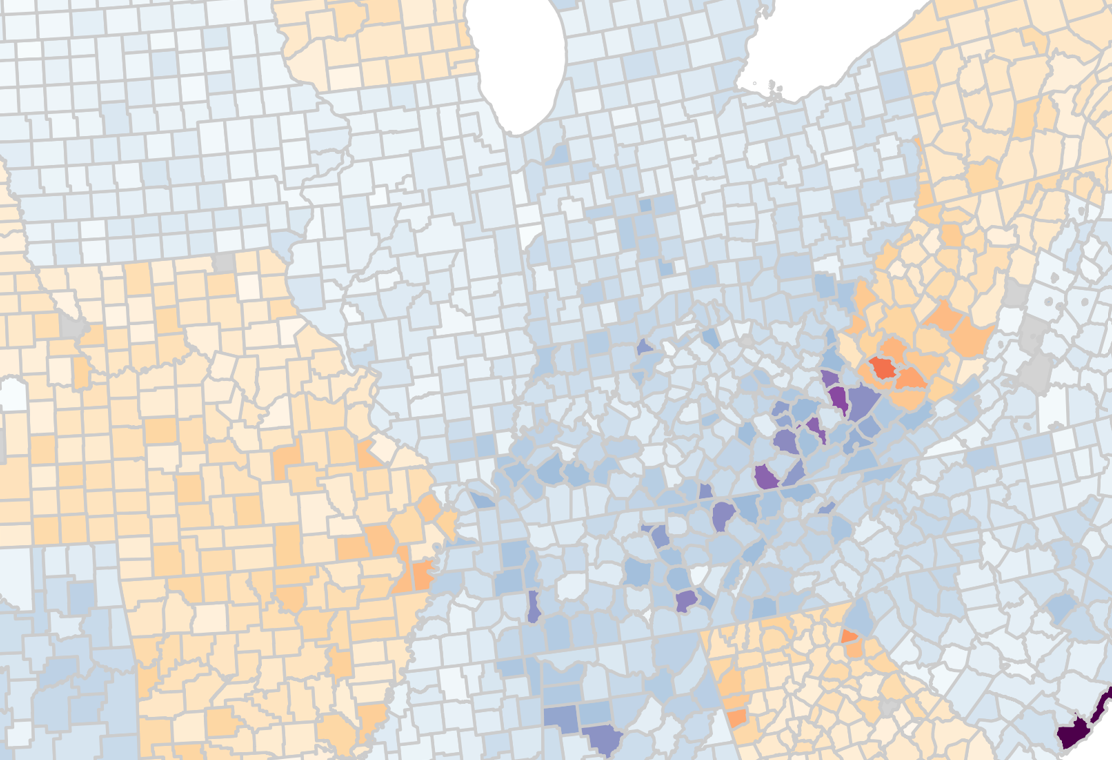
\includegraphics[scale=0.4]{thumbnail.png}}
    \end{center}
    
    %\hyperlink{}{\beamerbutton{Back}}
    
\end{frame}



\end{document}
